\section*{Answer 2}

Algorithm 5.1 of the textbook can be used to generate the weights of automobiles and trucks because the weights of them have Poisson distribution. The sample MATLAB code for automobiles:
\begin{myminted}
% automobiles
lambda = 50;      % parameter
U = rand;         % generated uniform variable
i = 0;            % initial value
F = exp(-lambda); % initial value of F(0)
while (U>=F)
  i = i + 1;
  F = F + exp(-lambda) * lambda^i / gamma(i+1);
end
n_a = i;          % total number of automobiles
\end{myminted}

Since the weight of each automobile and truck has a Gamma random variable, the formula from example 5.11 can be used. This value may be used to estimate the probability that the total weight of all the vehicles that pass over the bridge on a day is more than 200 tons.

\begin{myminted}
X = sum(-1/0.15 * log(rand(190,1))); % formula from example 5.11
\end{myminted}

This variable is valid for only 1 occurence. Therefore, it is necessary to calculate new variable $j$ times (number of automobiles or trucks) and sum them up.

\noindent By using the matlab code that is attached and provided (hw4.m);
\begin{itemize}
  \item The estimated probability of having the total weight of all the vehicles that pass over the bridge in a day more than 200 tons is \textbf{0.222437}
  \item The estimated total weight of all the vehicles that pass over the bridge in a day is \textbf{173632.748586} kilograms which is approximately \textbf{173.6} tons.
  \item The estimated Standard deviation is \textbf{35781.459393}. In this simulation $\alpha = 0.01$ and $\varepsilon = 0.02$ are used, so the study yields to accurate results within the error margin of $0.02$ and $0.99\%$ of the time.
  
  Since the theoretical Standard deviation is Std$(X) = \dfrac{\sigma}{\sqrt{N}}$, Std$(X)$ can be reduced by using the larger study sizes.
\end{itemize}

\noindent The screenshot of the output of \texttt{hw4.m},
\begin{figure}[ht]
  \centering
  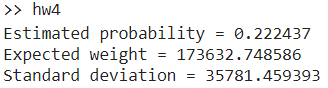
\includegraphics[width=.5\linewidth]{tex-files/hw4-results.png}
\end{figure}
